\documentclass[journal,12pt,twocolumn]{IEEEtran}
\usepackage{multicol}
\usepackage{blindtext}

\usepackage{graphicx}
\usepackage{setspace}
\usepackage{gensymb}
\singlespacing
\usepackage[cmex10]{amsmath}
\usepackage{amssymb}
\usepackage{xurl}
\usepackage{tabularx}
\usepackage{amsthm}
\usepackage{comment}
\usepackage{mathrsfs}
\usepackage{txfonts}
\usepackage{stfloats}
\usepackage{bm}
\usepackage{cite}
\usepackage{cases}
\usepackage{subfig}
\usepackage{arydshln}
\usepackage{longtable}
\usepackage{multirow}

\usepackage{enumitem}
\usepackage{mathtools}
\usepackage{steinmetz}
\usepackage{tikz}
\usepackage{circuitikz}
\usepackage{verbatim}
\usepackage{tfrupee}
\usepackage[breaklinks=true]{hyperref}
\usepackage{graphicx}
\usepackage{tkz-euclide}
\usetikzlibrary{automata, positioning}
\usetikzlibrary{calc,math}
\usepackage{listings}
    \usepackage{color}                                            %%
    \usepackage{array}                                            %%
    \usepackage{longtable}                                        %%
    \usepackage{calc}                                             %%
    \usepackage{multirow}                                         %%
    \usepackage{hhline}                                           %%
    \usepackage{ifthen}                                           %%
    \usepackage{lscape}     
\usepackage{multicol}
\usepackage{chngcntr}
\usepackage{blkarray}

\DeclareMathOperator*{\Res}{Res}

\renewcommand\thesection{\arabic{section}}
\renewcommand\thesubsection{\thesection.\arabic{subsection}}
\renewcommand\thesubsubsection{\thesubsection.\arabic{subsubsection}}

\renewcommand\thesectiondis{\arabic{section}}
\renewcommand\thesubsectiondis{\thesectiondis.\arabic{subsection}}
\renewcommand\thesubsubsectiondis{\thesubsectiondis.\arabic{subsubsection}}


\hyphenation{op-tical net-works semi-conduc-tor}
\def\inputGnumericTable{}                                 %%

\lstset{
%language=C,
frame=single, 
breaklines=true,
columns=fullflexible
}



\begin{document}


\newtheorem{theorem}{Theorem}[section]
\newtheorem{problem}{Problem}
\newtheorem{proposition}{Proposition}[section]
\newtheorem{lemma}{Lemma}[section]
\newtheorem{corollary}[theorem]{Corollary}
\newtheorem{example}{Example}[section]
\newtheorem{definition}[problem]{Definition}

\newcommand{\BEQA}{\begin{eqnarray}}
\newcommand{\EEQA}{\end{eqnarray}}
\newcommand{\define}{\stackrel{\triangle}{=}}
\bibliographystyle{IEEEtran}
\raggedbottom
\setlength{\parindent}{0pt}
\providecommand{\mbf}{\mathbf}
\providecommand{\pr}[1]{\ensuremath{\Pr\left(#1\right)}}
\providecommand{\qfunc}[1]{\ensuremath{Q\left(#1\right)}}
\providecommand{\sbrak}[1]{\ensuremath{{}\left[#1\right]}}
\providecommand{\lsbrak}[1]{\ensuremath{{}\left[#1\right.}}
\providecommand{\rsbrak}[1]{\ensuremath{{}\left.#1\right]}}
\providecommand{\brak}[1]{\ensuremath{\left(#1\right)}}
\providecommand{\lbrak}[1]{\ensuremath{\left(#1\right.}}
\providecommand{\rbrak}[1]{\ensuremath{\left.#1\right)}}
\providecommand{\cbrak}[1]{\ensuremath{\left\{#1\right\}}}
\providecommand{\lcbrak}[1]{\ensuremath{\left\{#1\right.}}
\providecommand{\rcbrak}[1]{\ensuremath{\left.#1\right\}}}
\theoremstyle{remark}
\newtheorem{rem}{Remark}
\newcommand{\sgn}{\mathop{\mathrm{sgn}}}
\providecommand{\abs}[1]{\vert#1\vert}
\providecommand{\res}[1]{\Res\displaylimits_{#1}} 
\providecommand{\norm}[1]{\lVert#1\rVert}
%\providecommand{\norm}[1]{\lVert#1\rVert}
\providecommand{\mtx}[1]{\mathbf{#1}}
\providecommand{\mean}[1]{E[ #1 ]}
\providecommand{\fourier}{\overset{\mathcal{F}}{ \rightleftharpoons}}
%\providecommand{\hilbert}{\overset{\mathcal{H}}{ \rightleftharpoons}}
\providecommand{\system}{\overset{\mathcal{H}}{ \longleftrightarrow}}
	%\newcommand{\solution}[2]{\textbf{Solution:}{#1}}
\newcommand{\solution}{\noindent \textbf{Solution: }}
\newcommand{\cosec}{\,\text{cosec}\,}
\providecommand{\dec}[2]{\ensuremath{\overset{#1}{\underset{#2}{\gtrless}}}}
\newcommand{\myvec}[1]{\ensuremath{\begin{pmatrix}#1\end{pmatrix}}}
\newcommand{\mydet}[1]{\ensuremath{\begin{vmatrix}#1\end{vmatrix}}}
\newcommand*{\permcomb}[4][0mu]{{{}^{#3}\mkern#1#2_{#4}}}
\newcommand*{\perm}[1][-3mu]{\permcomb[#1]{P}}
\newcommand*{\comb}[1][-1mu]{\permcomb[#1]{C}}
\numberwithin{equation}{subsection}
\makeatletter
\@addtoreset{figure}{problem}
\makeatother
\let\StandardTheFigure\thefigure
\let\vec\mathbf
\renewcommand{\thefigure}{\theproblem}
\def\putbox#1#2#3{\makebox[0in][l]{\makebox[#1][l]{}\raisebox{\baselineskip}[0in][0in]{\raisebox{#2}[0in][0in]{#3}}}}
     \def\rightbox#1{\makebox[0in][r]{#1}}
     \def\centbox#1{\makebox[0in]{#1}}
     \def\topbox#1{\raisebox{-\baselineskip}[0in][0in]{#1}}
     \def\midbox#1{\raisebox{-0.5\baselineskip}[0in][0in]{#1}}
\vspace{3cm}
\title{\textbf{LINEAR SYSTEMS AND SIGNAL PROCESSING \\ GATE ASSIGNMENT 2}}
\author{GANJI VARSHITHA - AI20BTECH11009}
\maketitle
\newpage
\bigskip
\renewcommand{\thefigure}{\arabic{figure}}
\renewcommand{\thetable}{\arabic{table}}
Download latex codes from 
%
\begin{lstlisting}
https://github.com/VARSHITHAGANJI/EE3900_GATE_ASSIGNMENTS/blob/main/GATE_ASSIGNMENT2/GATE_ASSIGNMENT2.tex
\end{lstlisting}
Download all python codes from
\begin{lstlisting}
https://github.com/VARSHITHAGANJI/EE3900_VECTORS_ASSIGNMENTS/blob/main/GATE_ASSIGNMENT2/code_graphs.py
\end{lstlisting}

\section*{QUESTION}
\textbf{GATE EC 2008- Q35}\\
Let x\brak{t} be the input and y\brak{t} be the output of a continuous time system. Match the system properties P1, P2, and P3 with the system relations R1, R2, R3, R4.
\begin{multicols}{2}


\textbf{Properties}\\
P1: Linear but NOT time-invariant\\
P2: Time-invariant but NOT linear\\
P3: Linear and time-invariant
\columnbreak

\textbf{Relations}\\
R1: y\brak{\text{t}} = $\text{t}^2\text{x}\brak{\text{t}}$ \\
\\
R2: y\brak{\text{t}} = $\text{t}| \text{x}\brak{\text{t}}|$ \\
\\
R3: y\brak{\text{t}} = $| \text{x}\brak{\text{t}}|$ \\
\\
R4: y\brak{\text{t}} = $\text{x}\brak{\text{t}-5}$ \\


\end{multicols}
\begin{enumerate}
\item \brak{\text{P1,R1}}, \brak{\text{P2,R3}}, \brak{\text{P3,R4}}
\item \brak{\text{P1,R2}}, \brak{\text{P2,R3}}, \brak{\text{P3,R4}}
\item \brak{\text{P1,R3}}, \brak{\text{P2,R1}}, \brak{\text{P3,R2}}
\item \brak{\text{P1,R1}}, \brak{\text{P2,R2}}, \brak{\text{P3,R3}}
\end{enumerate}
\section*{SOLUTION}
\begin{definition}
We say that a system is\textbf{ linear} if and only if it follows the Principle of Superposition, i.e Law of Additivity and Law of Homogeneity.
\label{L}
\end{definition}
\begin{definition}
A system is said to be \textbf{time invariant} if the output signal does not depend on the absolute time, i.e a time delay on the input signal directly equates to the delay in the output signal.
\label{T}
\end{definition}


\underline{Law of Additivity:}\\
Let the three input signals be $x_1(t)$, $x_2(t)$, and $x_1(t) + x_2(t)$  and their corresponding output signals be $y_1(t)$, $y_2(t)$, and $y'(t)$, then:
For R1:
\begin{align}
\label{eq:1}
    \text{y}_1\brak{\text{t}} ={}& \text{t}^2\text{x}_{1}\brak{\text{t}}\\
    \label{eq:2}
    \text{y}_2\brak{\text{t}}  ={}& \text{t}^2\text{x}_{1}\brak{\text{t}}\\
    \label{eq:3}
   \text{y}_1\brak{\text{t}} +\text{y}_2\brak{\text{t}}  ={}& \text{t}^2\brak{\text{x}_{1}\brak{\text{t}}+\text{x}_{2}\brak{\text{t}}}\\
   \label{eq:4}
 \text{y'}\brak{\text{t}} ={}& \text{t}^2\brak{\text{x}_{1}\brak{\text{t}}+\text{x}_{2}\brak{\text{t}}}
\end{align}
Clearly, from \eqref{eq:3} and \eqref{eq:4}:
\begin{align}
\label{eq:5}
    \text{y'}\brak{\text{t}} = \text{y}_1\brak{\text{t}} +\text{y}_2\brak{\text{t}} 
\end{align}
Thus, the Law of Additivity holds.\\
For R2:
\begin{align}
\label{eq:6}
    \text{y}_1\brak{\text{t}} ={}& \text{t}\; |\:\text{x}_{1}\brak{\text{t}}|\\
    \label{eq:7}
    \text{y}_2\brak{\text{t}}  ={}& \text{t}\;|\:\text{x}_{1}\brak{\text{t}}|\\
    \label{eq:8}
   \text{y}_1\brak{\text{t}} +\text{y}_2\brak{\text{t}}  ={}& \text{t}\;\brak{|\;\text{x}_{1}\brak{\text{t}}|+|\;\text{x}_{2}\brak{\text{t}}|}\\
   \label{eq:9}
 \text{y'}\brak{\text{t}} ={}& \text{t}\brak{|\;\text{x}_{1}\brak{\text{t}}+\text{x}_{2}\brak{\text{t}}|}
\end{align}
Clearly, from \eqref{eq:8} and \eqref{eq:9}:
\begin{align}
\label{eq:10}
    \text{y'}\brak{\text{t}} \leq \text{y}_1\brak{\text{t}} +\text{y}_2\brak{\text{t}} 
\end{align}
Thus, the Law of Additivity does not hold.\\
For R3:
\begin{align}
\label{eq:11}
    \text{y}_1\brak{\text{t}} ={}& |\:\text{x}_{1}\brak{\text{t}}|\\
    \label{eq:12}
    \text{y}_2\brak{\text{t}}  ={}& |\:\text{x}_{1}\brak{\text{t}}|\\
    \label{eq:13}
   \text{y}_1\brak{\text{t}} +\text{y}_2\brak{\text{t}}  ={}& \brak{|\:\text{x}_{1}\brak{\text{t}}|+|\:\text{x}_{2}\brak{\text{t}}|}\\
   \label{eq:14}
 \text{y'}\brak{\text{t}} ={}& \brak{|\;\text{x}_{1}\brak{\text{t}}+\text{x}_{2}\brak{\text{t}}|}
\end{align}
Clearly, from \eqref{eq:13} and \eqref{eq:14}:
\begin{align}
\label{eq:15}
    \text{y'}\brak{\text{t}} \leq \text{y}_1\brak{\text{t}} +\text{y}_2\brak{\text{t}} 
\end{align}
Thus, the Law of Additivity does not hold.\\

For R4:
\begin{align}
\label{eq:16}
    \text{y}_1\brak{\text{t}} ={}& \text{x}_{1}\brak{\text{t}-5}\\
    \label{eq:17}
    \text{y}_2\brak{\text{t}}  ={}& \text{x}_{1}\brak{\text{t}-5}\\
    \label{eq:18}
   \text{y}_1\brak{\text{t}} +\text{y}_2\brak{\text{t}}  ={}& \brak{\text{x}_{1}\brak{\text{t}-5}+\text{x}_{2}\brak{\text{t}-5}}\\
   \label{eq:19}
 \text{y'}\brak{\text{t}} ={}& \brak{\text{x}_{1}\brak{\text{t}-5}+\text{x}_{2}\brak{\text{t}-5}}
\end{align}
Clearly, from \eqref{eq:18} and \eqref{eq:19}:
\begin{align}
\label{eq:20}
    \text{y'}\brak{\text{t}} = \text{y}_1\brak{\text{t}} +\text{y}_2\brak{\text{t}} 
\end{align}
Thus, the Law of Additivity holds.\\



\underline{Law of Homogeneity: }\\
Consider an input signal $kx(t)$, where $k$ is any constant. Let the corresponding output be given by $y'(t)$, then:

For R1:
\begin{align}
\label{eq:21}
 \text{y'}\brak{\text{t}} ={}& \text{t}^2\text{k}\text{x}\brak{\text{t}}\\
 \label{eq:22}
   ={}& \text{k}\text{y}\brak{\text{t}}
\end{align}
Clearly, from \eqref{eq:22}:
\begin{align}
\label{eq:23}
    \text{y'}\brak{\text{t}} ={}& \text{k}\text{y}\brak{\text{t}}
\end{align}
Thus, the Law of homogeneity holds.\\

For R2:
\begin{align}
\label{eq:24}
 \text{y'}\brak{\text{t}} ={}& \text{t}|\:\text{k}\text{x}\brak{\text{t}}|\\
 \label{eq:25}
   ={}& |\:\text{k}|\text{y}\brak{\text{t}}
\end{align}
Clearly, from \eqref{eq:25}:
\begin{align}
\label{eq:26}
    \text{y'}\brak{\text{t}} \neq{}& \text{k}\text{y}\brak{\text{t}}
\end{align}
Thus, the Law of homogeneity does not hold.\\

For R3:
\begin{align}
\label{eq:27}
 \text{y'}\brak{\text{t}} ={}& |\:\text{k}\text{x}\brak{\text{t}}|\\
 \label{eq:28}
   ={}& |\:\text{k}|\text{y}\brak{\text{t}}
\end{align}
Clearly, from \eqref{eq:28}:
\begin{align}
\label{eq:29}
    \text{y'}\brak{\text{t}} \neq{}& \text{k}\text{y}\brak{\text{t}}
\end{align}
Thus, the Law of homogeneity does not hold.\\

For R4:
\begin{align}
\label{eq:30}
 \text{y'}\brak{\text{t}} ={}& \text{k}\text{x}\brak{\text{t}-5}\\
 \label{eq:31}
   ={}& \text{k}\text{y}\brak{\text{t}}
\end{align}
Clearly, from \eqref{eq:31}:
\begin{align}
\label{eq:32}
    \text{y'}\brak{\text{t}} ={}& \text{k}\text{y}\brak{\text{t}}
\end{align}
Thus, the Law of homogeneity holds.\\
$\therefore$ We get R1 and R4 are linear systems whereas R2 and R3 are non linear systems.\\
\\
To check time-invariance, we introduce a delay of $\text{t}_{0}$ in the output and input signal.Let the delayed output signal is $\text{y}\brak{\text{t}-\text{t}_{0}}$ and the output signal corresponding to the input signal delayed by $\text{t}_{0}$ is given by $\text{y'}\brak{\text{t}}$.\\
For R1:
\begin{align}
\label{eq:33}
 \text{y}\brak{\text{t}-\text{t}_{0}} ={}& \brak{\text{t}-\text{t}_{0}}^2\text{x}\brak{\text{t}-\text{t}_{0}}\\
 \label{eq:34}
  \text{y'}\brak{\text{t}}={}& \brak{\text{t}}^2\text{x}\brak{\text{t}-\text{t}_{0}}
\end{align}
Clearly, from \eqref{eq:33} and \eqref{eq:34}:
\begin{align}
\label{eq:35}
    \text{y}\brak{\text{t}-\text{t}_{0}} \neq{}& \text{y'}\brak{\text{t}}
\end{align}
Thus, the system is not time invariant.\\
For R2:
\begin{align}
\label{eq:36}
 \text{y}\brak{\text{t}-\text{t}_{0}} ={}& \brak{\text{t}-\text{t}_{0}}|\;\text{x}\brak{\text{t}-\text{t}_{0}}|\\
 \label{eq:37}
  \text{y'}\brak{\text{t}}={}& \brak{\text{t}}|\;\text{x}\brak{\text{t}-\text{t}_{0}}|
\end{align}
Clearly, from \eqref{eq:37} and \eqref{eq:38}:
\begin{align}
\label{eq:38}
    \text{y}\brak{\text{t}-\text{t}_{0}} \neq{}& \text{y'}\brak{\text{t}}
\end{align}
Thus, the system is not time invariant.\\
For R3:
\begin{align}
\label{eq:39}
 \text{y}\brak{\text{t}-\text{t}_{0}} ={}& |\;\text{x}\brak{\text{t}-\text{t}_{0}}|\\
 \label{eq:40}
  \text{y'}\brak{\text{t}}={}& |\;\text{x}\brak{\text{t}-\text{t}_{0}}|
\end{align}
Clearly, from \eqref{eq:39} and \eqref{eq:40}:
\begin{align}
\label{eq:41}
    \text{y}\brak{\text{t}-\text{t}_{0}} ={}& \text{y'}\brak{\text{t}}
\end{align}
Thus, the system is time invariant.\\
For R4:
\begin{align}
\label{eq:42}
 \text{y}\brak{\text{t}-\text{t}_{0}} ={}& \text{x}\brak{\text{t}-\text{t}_{0}-5}\\
 \label{eq:43}
  \text{y'}\brak{\text{t}}={}& \text{x}\brak{\text{t}-\text{t}_{0}-5}
\end{align}
Clearly, from \eqref{eq:42} and \eqref{eq:43}:
\begin{align}
\label{eq:44}
    \text{y}\brak{\text{t}-\text{t}_{0}} ={}& \text{y'}\brak{\text{t}}
\end{align}
Thus, the system is time invariant.\\

$\therefore$ We get R3 and R4 are time invariant systems whereas R1 and R2 are not time invariant. 

Tabulating the results,
\\
\begin{table}[h]
\label{table:questions}
\begin{tabular}{ |m{1.5cm}|m{2cm}|m{2.5cm}| } 
 \hline
 System & Linear & Time invariant \\ 
 \hline
R1 & Yes & No\\[1ex]
 \hline
 R2 & No & No\\[1ex]
 \hline
 R3 & No & Yes\\[1ex]
 \hline
 R4 & Yes & Yes\\[1ex]
 \hline
\end{tabular}

\end{table}\\
From the above table , option (1) is correct.

Verification using simple signals.\\

\begin{figure}[h]
\caption{Input signals}
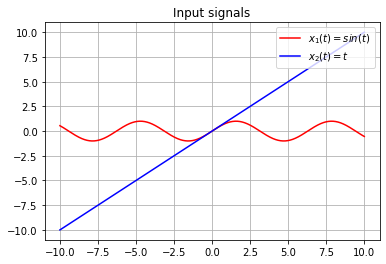
\includegraphics[width = \columnwidth]{input}
\end{figure}


\begin{figure}[h]
\caption{R1 system: y\brak{\text{t}} = $\text{t}^2\text{x}\brak{\text{t}}$ }
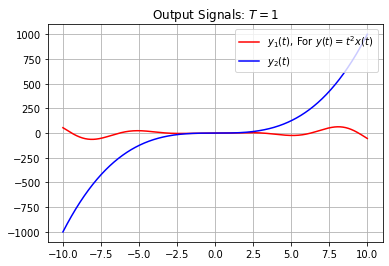
\includegraphics[width = \columnwidth]{y1}
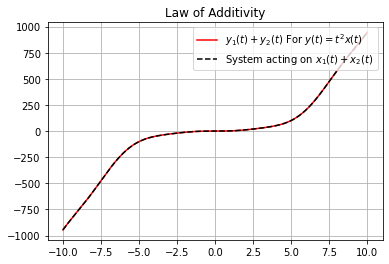
\includegraphics[width = \columnwidth]{y1_p}

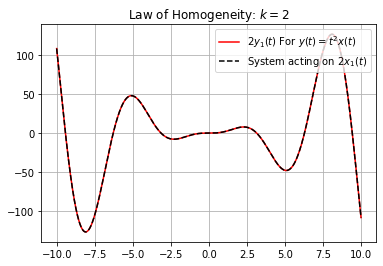
\includegraphics[width = \columnwidth]{y1_h}

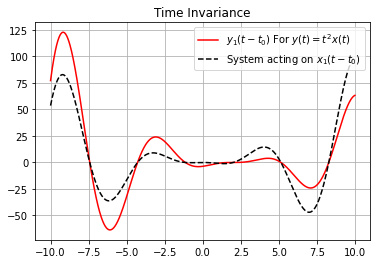
\includegraphics[width = \columnwidth]{y1_t}
\end{figure}



\begin{figure}[h]
\caption{R2 system: y\brak{\text{t}} = $\text{t}|\; \text{x}\brak{\text{t}}|$}
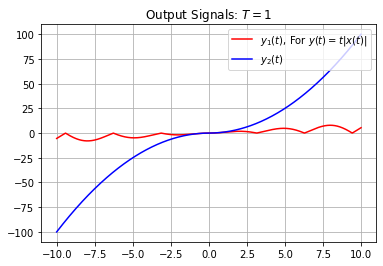
\includegraphics[width = \columnwidth]{y2}
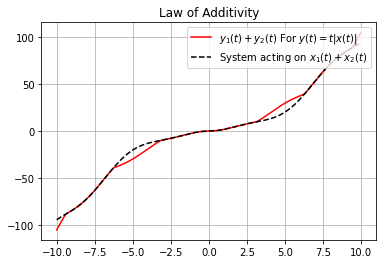
\includegraphics[width = \columnwidth]{y2_p}

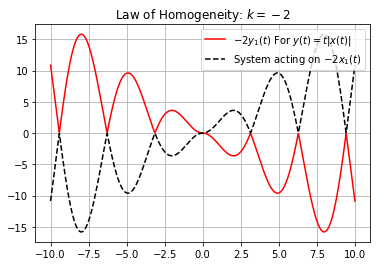
\includegraphics[width = \columnwidth]{y2_h}

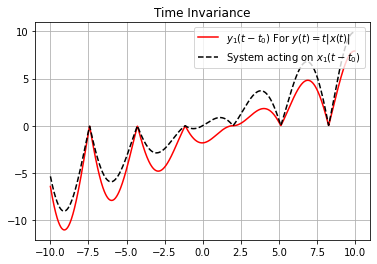
\includegraphics[width = \columnwidth]{y2_t}
\end{figure}



\begin{figure}[h]
\caption{R3 system: y\brak{\text{t}} = $|\;\text{x}\brak{\text{t}}|$}
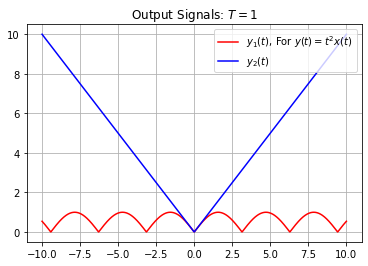
\includegraphics[width = \columnwidth]{y3}
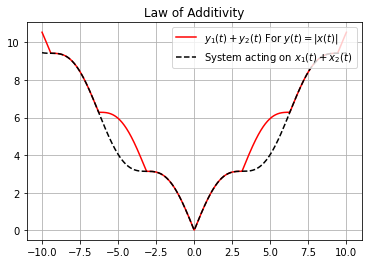
\includegraphics[width = \columnwidth]{y3_p}

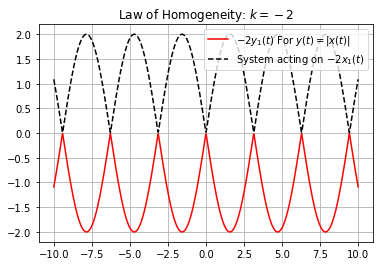
\includegraphics[width = \columnwidth]{y3_h}

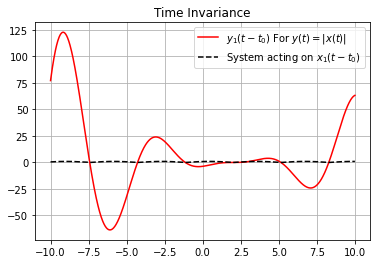
\includegraphics[width = \columnwidth]{y3_t}
\end{figure}



\begin{figure}[h]
\caption{R4 system: y\brak{\text{t}} = $\text{x}\brak{\text{t-5}}$}
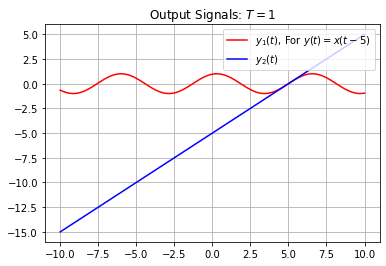
\includegraphics[width = \columnwidth]{y4}
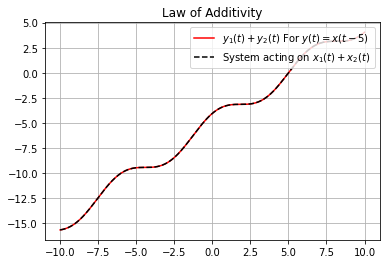
\includegraphics[width = \columnwidth]{y4_p}

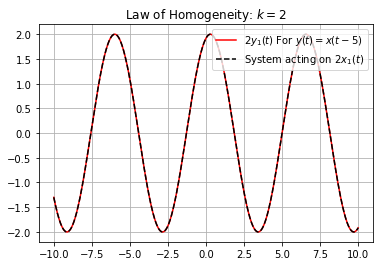
\includegraphics[width = \columnwidth]{y4_h}

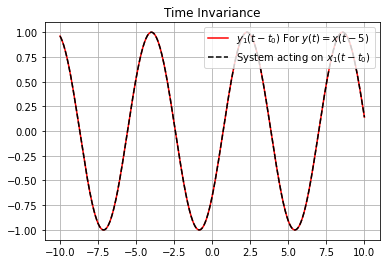
\includegraphics[width = \columnwidth]{y4_t}
\end{figure}










\end{document}
